\documentclass[conference]{IEEEtran}
\IEEEoverridecommandlockouts
% The preceding line is only needed to identify funding in the first footnote. If that is unneeded, please comment it out.
\usepackage{cite}
\usepackage{amsmath,amssymb,amsfonts}
\usepackage{algorithmic}
\usepackage{graphicx}
\usepackage{textcomp}
\usepackage{xcolor}
\usepackage{float}
\def\BibTeX{{\rm B\kern-.05em{\sc i\kern-.025em b}\kern-.08em
    T\kern-.1667em\lower.7ex\hbox{E}\kern-.125emX}}
\begin{document}

\title{HOMEWOEK 3}

\author{\IEEEauthorblockN{Runlin Hou}
\IEEEauthorblockA{\textit{ECE, School Of Graduate Studies} \\
\textit{Rutgers University}\\
hourunlinxa@gmail.com}
}

\maketitle

\section*{Question 1}
The given graph is not acycilc, since I detected a cycle in the graph. 

\section*{Question 2}
The weights of MST decided by the are the same which is 10.46351.

\begin{figure}[H]
    \centerline{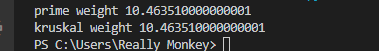
\includegraphics[scale=0.8]{pic/pic2.png}}
    \caption{Topological Sort}
\end{figure}

The time consumption of the two alogirithms are show below,

\begin{table}[H]
    \begin{center}
        \begin{tabular}{|l|l|l|}
            \hline
            \textbf{}     & prime & kruskal \\ \hline
            \textbf{Time} & 0.069 & 0.002   \\ \hline
            \end{tabular}
    \end{center}
\end{table}

We can see that the time consumption of kruskal is much smaller than 
the prime alogirithm. The reason is that the idea of prime algorithm 
if to find the edge that is already in the marked edges, so it will 
take much more traversal. The kruskal is different that it only traverse 
the edges once to find the smallest edges.

\section*{Question 3}

We find the topological sort of this graph and shown as below,

\begin{figure}[H]
    \centerline{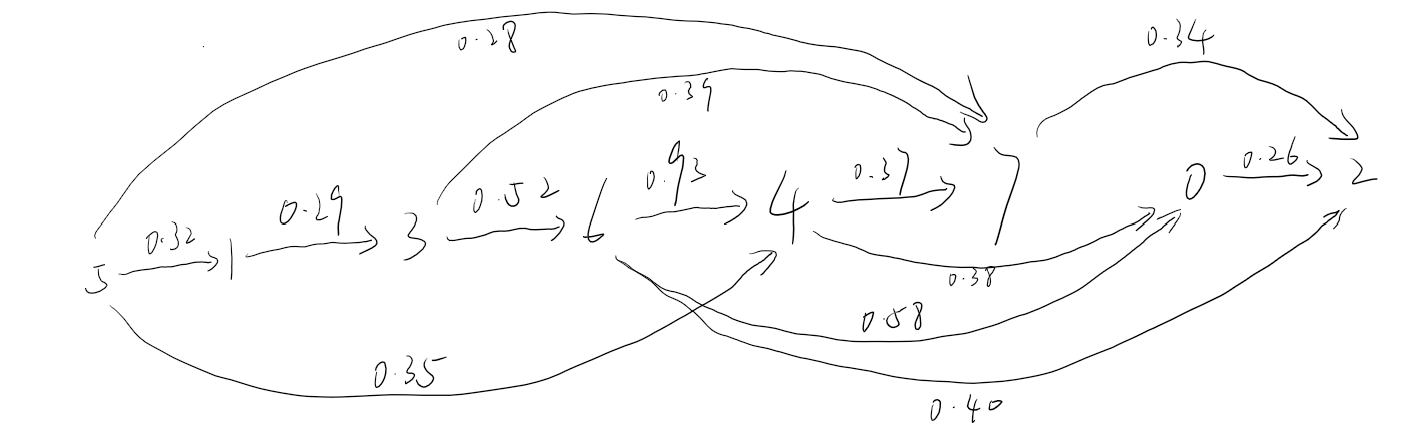
\includegraphics[scale=0.5]{pic/pic1.png}}
    \caption{Topological Sort}
\end{figure}

Now according to the topological sort of the graph, we can compute 
the longest path from 5 to every vertice.

\begin{table}[H]
    \caption{}
    \begin{center}
        \begin{tabular}{|c|c|c|c|c|c|c|c|c|}
            \hline
            &0&1&2&3&4&5&6&7\\
            \hline
            edgeTo()&4-0&5-1&7-2&1-3&6-4&null&3-6&4-7\\
            \hline
            disTo()&2.44&0.32&2.77&0.61&2.06&0&1.13&2.43\\
            \hline
        \end{tabular}
    \end{center}
\end{table}

Also, from the topological sort we can get the shortest path from 5.

\begin{table}[H]
    \caption{}
    \begin{center}
        \begin{tabular}{|c|c|c|c|c|c|c|c|c|}
            \hline
            &0&1&2&3&4&5&6&7\\
            \hline
            edgeTo()&4-0&5-1&7-2&1-3&5-4&null&3-6&5-7\\
            \hline
            disTo()&0.73&0.32&0.62&0.61&0.35&null&1.13&0.28\\
            \hline
        \end{tabular}
    \end{center}
\end{table}

\section*{Question 4}
By Bellman-Ford alogirithm, I choose 0 to be the starter vertice and 
initial all the distence to be $\infty$

\begin{table}[H]
    \begin{center}
        \begin{tabular}{|c|c|c|c|c|c|c|c|c|}
            \hline
            \textbf{}    & 0 & 1    & 2    & 3    & 4    & 5    & 6    & 7    \\ \hline
            \textbf{Ini} & 0 & $\infty$ & $\infty$ & $\infty$ & $\infty$ & $\infty$ & $\infty$ & $\infty$ \\ \hline
            \textbf{1st} & 0 & 1.05 & 0.26 & 0.99 & 0.38 & 0.73 & $\infty$ & 0.60 \\ \hline
            \textbf{2nd} & 0 & 1.05 & 0.26 & 0.99 & 0.26 & 0.73 & 1.51 & 0.60 \\ \hline
            \textbf{3rd} & 0 & 1.05 & 0.26 & 0.99 & 0.26 & 0.61 & 1.51 & 0.60 \\ \hline
            \textbf{4th} & 0 & 0.93 & 0.26 & 0.99 & 0.26 & 0.61 & 1.51 & 0.60 \\ \hline
            \textbf{5th} & 0 & 0.93 & 0.26 & 0.99 & 0.26 & 0.61 & 1.51 & 0.60 \\ \hline
            \end{tabular}
    \end{center}
\end{table}

As we can see that the 5th iteratoin doest not change any value, so that we can
stop here since there is not going to be any changes.

\begin{table}[H]
    \begin{center}
        \begin{tabular}{|c|c|c|c|c|c|c|c|c|}
            \hline
            \textbf{}    & 0 & 1    & 2    & 3    & 4     & 5    & 6    & 7    \\ \hline
            \textbf{Ini} & 0 & $\infty$ & $\infty$ & $\infty$ & $\infty$ & $\infty$ & $\infty$ & $\infty$ \\ \hline
            \textbf{1st} & 0 & 1.05 & 0.26 & 0.99 & 0.07  & 0.73 & $\infty$ & 0.60 \\ \hline
            \textbf{2nd} & 0 & 0.74 & 0.26 & 0.83 & -0.24 & 0.42 & 1.51 & 0.44 \\ \hline
            \textbf{3rd} & 0 & 0.43 & 0.26 & 0.52 & -0.55 & 0.11 & 1.35 & 0.13 \\ \hline
            $\cdots$ & $\cdots$&$\cdots$ &$\cdots$ &$\cdots$ & $\cdots$ & $\cdots$ & $\cdots$ & $\cdots$ \\ \hline
            \end{tabular}
    \end{center}
\end{table}

We can find that the distence will keep falling, since 4 and 5 can reduce each other in each iteratoin.
This will always happen when there is a negative circle inside the graph.

\subsection*{Question 5}

Before I implement DFS and BFS, I first create the graph based on the network of NYC. 
Since we just have to do the traversal of the graph, I ignore the weights of the graph.
And the structure of the graoh is a list who saves the adjacencies of each vertice and 
the vertice can be directed by its index.

For the implementation of DFS, I'm using recursion to achieve the algorithm. We will reach 
the input vertice's child before we reach its other brothers and each time we reach a vertice 
it will be marked and won't be visit again. The recursion will end when there is no vertex to 
be visited. Something we need to notice is that when we are using python to implement this alogirithm
we may reach the threshold of the recursion, so we may need to use \verb|sys.setresionlimit()| to avoid
hitting the upper bound.

BFS can be implement without recursion. I use nested loops to ahieve our goal. Also we need a queue
to save the incoming vertice. When reach a vertice, its children will be added to the tail of the 
queue and the vertice itself will be removed and marked visited. We there is no vertice in the queue
, we end our loop.

\subsection*{Question 6}



\end{document}
